\documentclass[12pt]{extarticle}
\usepackage[utf8]{inputenc}
\usepackage[margin=1in]{geometry}

\usepackage[cmintegrals,cmbraces]{newtxmath}
%\usepackage{ebgaramond}

\usepackage{amsmath}
\usepackage{amsfonts}
%\usepackage{amssymb}

%table numbers within section
\usepackage{chngcntr}
\counterwithin{table}{section}

\usepackage{natbib}
\usepackage{graphicx}
\usepackage{booktabs}
\usepackage{longtable}
\usepackage{caption}

%\frenchspacing
\usepackage{setspace}
\setstretch{1.1}

\usepackage{graphicx}
\usepackage{url}
\usepackage[colorlinks=true, urlcolor = orange, linkcolor=blue, citecolor=purple]{hyperref}

\usepackage{xcolor}
%\usepackage{sectsty}
\usepackage{appendix}

%\subsectionfont{\color{cyan!70!blue}}  % sets colour of chapters
%\sectionfont{\color{blue!60!black}}  % sets colour of sections

%Tables:
\usepackage{dcolumn}
\usepackage{float}
\usepackage{caption}
\usepackage{tabularx}

% Landscape mode
\usepackage{lscape}

% Modelsummary
\usepackage{threeparttable}
\usepackage{booktabs}
\usepackage{siunitx}
%\newcolumntype{d}{S[input-symbols = ()]}
\newcolumntype{d}{S[
    input-open-uncertainty=,
    input-close-uncertainty=,
    parse-numbers = false,
    table-align-text-pre=false,
    table-align-text-post=false
 ]}

\title{Institutions and Innovation: \\ Evidence from the Italian Unification\footnote{We thank Francesco Cinnirella for sharing municipality-level patent data for Italy, 1863-1867 and 1878, and Michelangelo Vasta for sharing patent data for 1902. We thank Bob Fahre for sharing the Trade Agreements Database.
We are grateful to the participants of the 2024 Utrecht PPE Conference, the 2024 Utrecht Applied Economics Seminar and the Ninth ASE Annual Meeting (2024) for insightful comments and suggestions. 
}
}
\author{Giacomo Domini \and Bas Machielsen\footnote{Both Utrecht University School of Economics, Utrecht University, Kriekenpitplein 21-22, 3584 EC Utrecht, the Netherlands; e--mail: \href{mailto:g.domini@uu.nl}{g.domini@uu.nl}, \href{mailto:a.h.machielsen@uu.nl}{a.h.machielsen@uu.nl}}}
\date{\today}

\begin{document}

\maketitle

%\begin{center}
%    For the latest version, please \href{http://link.com/paper.pdf}{click here.}
%\end{center}

\vspace{1 cm}

\begin{center} 
[PRELIMINARY: PLEASE DO NOT CITE OR CIRCULATE WITHOUT PERMISSION]

\vspace{1 cm}

\textbf{Abstract:} 
\end{center}

\noindent Economists have long acknowledged the centrality of innovation in economic growth and of institutions, defined as the “rules of the game”, as a determinant of innovation outcomes. 
This paper studies the impact on innovation of an important historical episode of institutional change, from the Italian unification process. 
We leverage quasi-random variation in the establishment of a new border after a war between Piedmont and Austria in 1859; and argue that the Western part of the Lombardo-Venetian Kingdom, which was annexed by Piedmont, was exposed to more liberal institutions than the Eastern part, which remained under Austria. 
We measure innovation using  patent data from Italy and Austria, as well as data from the universal exhibitions taking place in Paris in 1855, 1867, 1878, 1889, and 1900. 
Results from a regression-discontinuity design show a positive effect of the new institutional setting on either measure of innovation.

\bigskip
\textbf{JEL Classifications:} N14, D74, O31 % D72, H71

\textbf{Keywords:} Institutions; innovation; patents; Italian unification


\clearpage

\section{Introduction}

\noindent Economists have long seen innovation as the engine of economic growth \citep{schumpeter1942, solow1957}. 
Yet innovation is only a proximate cause for economic growth and itself an outcome to be explained by more fundamental causes. 
Institutions, defined as the “rules of the game”, are widely regarded as a primary determinant of innovation outcomes \citep{north1973, north1990, acemoglu2005}.\footnote{The importance of institutional frameworks in supporting innovative activities is also emphasized by the literature on national innovation systems, started by \citet{freeman1987} and further developed by \citet{lundvall1992} and \citet{nelson1993}.
}  
The stress lies primarily on \textit{inclusive} institutions, which enforce property rights for a large share of the population and guarantee some degree of equality of opportunity, as opposed to \textit{extractive} institutions, which miss these conditions and thus favour rent extraction by a limited amount of privileged people \citep{acemoglu2001, acemoglu2012}.\footnote{Not all scholars agree on the primary role of such institutions for growth: notably, \citet[][pp. 28-29]{allen2011} remarks that the taxation was higher and property rights were less protected in England than in France, yet it was the former that first industrialised.
}

While the relationship between institutions and innovation has been attracting increasing academic interest in the last two decades \citep[see][Figure 1]{he2020}, historical evidence is scarce \citep{donges2022}.
However, the past offers valuable cases of institutional change that can shed light on this topic. 
In particular, nineteenth-century Europe is fertile ground: on the one hand, the continent was swept by nationalist movements and demands for political and social reform. 
On the other hand, that century first saw, in its first half, the spread of the First Industrial Revolution to the continent and then the emergence of the Second Industrial Revolution. 

This paper focuses on an episode from Italy’s unification process in the 1850s and 1860s, namely the annexation of Lombardy to Piedmont from Austria, which we argue entailed a substantial shift towards liberal institutions, driven by quasi-random military circumstances. 
This institutional shock was the outcome of the Second War of Independence (1859), fought by Piedmont (formally the Kingdom of Sardinia) and France against Austria, with the intent to take from the latter the Lombardo-Venetian Kingdom, broadly corresponding to the present-day regions of Lombardy, Veneto, and Friuli. 
The eventual outcome of the war was that only the Western part of the Kingdom, namely Lombardy, was taken from Austria, as France --- to the dismay of Piedmont --- unexpectedly signed an armistice after the Franco-Piedmontese army achieved a decisive victory in Solferino, close to the border between Lombardy and Veneto. 

We argue that this unanticipated quasi-random establishment of a new border caused Lombardy to be ``treated'' with more liberal institutions, as it joined Piedmont, the most liberal state of Italy at that time, while Veneto remained under absolutist Austria. 
Indeed, Piedmont was the only Italian state not to repeal the constitution it had granted during the 1848 revolutions, known as \textit{Statuto Albertino} (from the name of king Carlo Alberto). 
This, which became the constitution of the unified Kingdom of Italy when the latter was proclaimed in 1861, was an advanced liberal constitution  for that time, %establishing an elective lower chamber (while the upper one was appointed), and 
enshrining the principles of equality before the law, individual liberty, freedom of press, and inviolability of private property.
Instead, Austria repealed its constitution in 1851 %--- marking the start of a period known as \textit{neo-absolutism} --- %
and only re-introduced one after the loss of Lombardy, which was still less liberal than Piedmont/Italy's \textit{Statuto}. 
In 1864, the liberal paper \textit{Wanderer} described Austria's constitution holding between 1861 and 1865, known as the February Patent, as  ``a constitution without freedom of association, without jury courts, without freedom of press, without equality of confessional rights, lacking a reform of justice and administration.”\footnote{\textit{Wanderer} No 361, dated 21st December 1841, Morgenblatt 1, as cited in \citet{olechowski2010}.
}

In line with the strand of literature mentioned above, we hypothesize that Piedmont/Italy's more liberal constitution may have provided a better institutional framework, encouraging innovation in the newly acquired territories. %s by establishing stronger individual and property rights. 
However, this was not the only dimension of the ``treatment'' Lombardy was subjected to, which might affect the innovation performance of that region.
A direct influence might have been exerted by the change from the Austrian to the Piedmontese patent system. 
In this regard, we notice that both were French-inspired registration-based systems involving no novelty examination. 
The fees to be paid by applicants were lower on the Italian side, but the difference depended on the duration requested, ranging from a minimum of zero to around one fourth. 
In the analysis below, we also discuss the potential effects of other changes associated with the annexation of Lombardy to Piedmont, notably those in market access and in the cultural homogeneity of the state, both of which are \textit{a priori} ambiguous.


Our empirical approach leverages the quasi-random assignment of the new border in a regression-discontinuity (RD) design. %, which relies on a parallel trends assumption, while absorbing level differences in the innovation of the two regions, prior to their division. 
%We combine DD with a regression-discontinuity (RD) approach, restricting the sample to areas sufficiently close to the border, which should strengthen the credibility of the parallel trends assumption.%; as well as cross-sectional RD regressions, which however rely on different --- and in our opinion less credible --- assumptions. 
We measure innovation by means of two sources, namely patents and the products displayed at the international exhibition held in Paris in 1855, 1867, 1878, 1889, and 1900. %, and in Turin in 1911. 
In this way, we hope to capture innovative activities to a greater extent, as \citet{domini2019} noticed that these two proxies suffer from opposite shortcomings. As for the former source, we sum Austrian and Piedmontese (Italian, after 1861) patents to account for the diversion of patenting activity, as Lombardy moved from one state to the other. %This is not a concern for the latter source, since we use data from the universal exhibitions taking place in a third country, namely France, in 1855, 1867, 1878, 1889, and 1900.

We conduct separate short- and long-run analyses. The former relies on yearly patent data for the period around the shock, namely 1855 to 1866 --- the year in which also Veneto joined the Kingdom of Italy. Long-run analyses are instead run on both patent and exhibition data at approximately decadal intervals between 1855 and 1900. %1911. 
Our results show that Veneto fell behind Lombardy in terms of either measure of innovation, in the years in which it remained under absolutist Austria while the neighbouring region joined liberal Piedmont/Italy. However, the gap vanished after Veneto also joined the Kingdom of Italy and was thus exposed to the same institutional setting.  
%It is important to mention that event studies do not reveal pre-trends, which lends credibility to the parallel trends assumption, underpinning the DD design.}

%[SOC. REL.; MOVE WHERE FIT] The historical analysis of this episode is particularly relevant in the current context, where the liberal-democratic global order faces serious challenges.

%\subsection*{Related literature}
Our study relates to the large empirical literature on the link between institutions, innovation, and economic growth. While earlier contributions do exist \citep[for instance,][show a negative association between absolutist rule and city growth in the pre-industrial era]{delong1993}, this literature has received as significant impulse from the seminal works by \citet{acemoglu2001, acemoglu2002} on the long-term effects of the different institutions sown by European colonisers around the world, also because of their influential instrumental-variable approach for causal inference. 
Similar evidence on the role of institutional quality in a large present-day cross section was soon after provided by \citet{rodrik2004} and \citet{aghion2007}.\footnote{See \citet{acemoglu2019} for further evidence on the positive effect of democracy on growth and an extensive review of the literature on that topic.
}
The latter pointed out that democratic institutions stimulated growth primarily by favouring market entry and thus innovation. 
\citet{gao2017} called the idea that democracy fosters innovation the ``Popper hypothesis'', as they traced it back to Karl Popper, but found no evidence for it. 
Instead \citet{wang2021} found robust evidence of a positive impact of democracy on patents and trademarks. 

Fewer studies specifically investigated the direct effect of institutions on innovation in historical settings. 
Some contributions provide evidence on the impact of differences in (the strenght of) patent systems on innovation, observing that the direction, rather than the rate of innovation, was affected \citep{moser2005, moser2012, lerner2009}.
\citet{greif2012} document the role of a social institution, namely the Old Poor Law introduced in 17-th century England, in favouring innovation at the time of the Industrial Revolution, by decreasing social unrest.
\cite{buonanno2024} provide evidence of the importance of institutions facilitating access to useful knowledge. They show that the 1866 expropriation of monastic properties in the Kingdom of Italy and the consequent increase in accessibility to the knowledge their libraries used to keep, had a positive causal effect on innovation in the following decades. 
The closest paper to our own is \citet{donges2022}, identifying a positive effect of the inclusive institutions brought by the French to German counties occupied during the Napoleonic era (including the dissolution of guilds, the introduction of the \textit{Code civil}, the abolition of serfdom, and agrarian reforms) on patenting. This paper is also similar in that it exploits for identification variation (in the duration of the French occupation) introduced by exogenous military and geopolitical factors.
We expand this literature by providing further micro-level evidence from historical shock previously unresearched for this purpuse. 

We also intend to contribute to the economic-history literature analysing the innovation performance of Italy in the very long run \citep{barbielliniamidei2013, nuvolari2015b}, in particular those making use of disaggregated datasets at the province level \citep{nuvolari2018}, municipality level \citep{buonanno2024}, firm level \citep{domini2023}, and entrepreneur level \citep{toninelli2014, nuvolari2018}. 
Most of these papers go back in time to the first post-unification years at the earliest, also due to the absence of a common patent system until then \citep{nuvolari2019}, with few exceptions going back to the pre-unification period \citep{nuvolari2020}. 
We add further evidence for a period starting before the unification. \footnote{Notice that the availability of data for such a distant time is remarkable by international standards, with the exception of the United States \citep{bergeaud24, petralia16}.}
%\textcolor{red}{[ALSO RELATE TO THE HISTORICAL LITERATURE ON ITALIAN REGIONAL DIVIDES?]}

\section{Historical background}

\subsection{The Lombardo-Venetian Kingdom}
As the Congress of Vienna (1814-1815) drew the borders of post-Napoleonic Europe, Austria organised its Northern Italian possessions (excluding Trento, which became part of the County of Tyrol) into a new state, the Lombardo-Venetian Kingdom.\footnote{It should also be noticed that branches of the Habsburg House were also ruling the Duchy of Modena and the Grand-Duchy of Tuscany.}
As the name suggests, this was a merger between two  regions with their own distinct histories. 
On the one hand, the Lombard territories of the former duchies of Milan and Mantua had been a Habsburg possession since the early 18th century. 
On the other hand, the Eastern part of the newly-established kingdom was the mainland of the former Republic of Venice, whose millennial history was terminated by the Treaty of Campoformio (1797), partitioning the lands of the republic between France and Austria. 
These also included Bergamo and Brescia, which became administratively part of Lombardy under the Lombardo-Venetian Kingdom.

On the verge of the 1859 war, the two regions were quite similar, in terms of summary economic development indicators. Lombardy was more populated than Veneto (2.8 vs 2.3 million inhabitants in 1857) despite a smaller surface (2.1 vs 2.4 million hectares). The two halves of the kingdom, however, had similar shares of agricultural population, only few percentage points higher in Lombardy, as shown in Table~\ref{tab:population_comp}. One should remark, however, that Veneto had a considerably larger agricultural population share in the early 1820s, revealing that structural transformation was faster in the East than in the West, in the four decades of life of the Lombardo-Venetian Kingdom.  

\begin{table}[!h]
\caption{\label{tab:population_comp}The Lombardo-Venetian provinces, 1857, \%}
\centering
%\fontsize{9}{11}\selectfont

    \begin{tabular}{l r r r r r r}  
        \toprule
        Province & Pop. & Pop./Ha & Urb. & Agr. & Ind. & Serv.    \\ 
        \midrule
        Bergamo & 0.39 & 0.98 & 0.07 & 0.68 & 0.17 & 0.15 \\
        \textit{Brescia} & 0.36 & 1.16 & 0.12 & 0.54 & 0.23 & 0.23 \\
        Como & 0.44 & 1.60 & 0.04 & 0.71 & 0.16 & 0.13 \\
        Cremona & 0.21 & 1.57 & 0.14 & 0.59 & 0.22 & 0.19 \\
        Lodi e Crema & 0.22 & 1.90 & 0.08 & 0.60 & 0.21 & 0.2 \\
        \textit{Mantova} & 0.26 & 1.13 & 0.11 & 0.65 & 0.19 & 0.16 \\
        Milano & 0.48 & 2.59 & 0.29 & 0.64 & 0.18 & 0.19 \\
        Pavia & 0.18 & 1.80 & 0.16 & 0.60 & 0.21 & 0.19 \\
        Sondrio & 0.10 & 0.32 & .00 & 0.76 & 0.13 & 0.11 \\
        \textbf{Lombardy} & 2.66 & 1.45 & 0.11 & 0.64 & 0.19 & 0.17 \\
         &  & &  &  &  \\
        Belluno & 0.15 & 0.48 & 0.07 & 0.72 & 0.18 & 0.10 \\
        Padova & 0.31 &1.45 & 0.18 & 0.57 & 0.29 & 0.15 \\
        Rovigo & 0.17 & 1.58 & 0.07 & 0.65 & 0.23 & 0.13 \\
        Treviso & 0.30 & 1.23 & 0.07 & 0.71 & 0.16 & 0.13 \\
        Udine & 0.43 & 0.65 & 0.05 & 0.70 & 0.19 & 0.11 \\
        Venezia & 0.30 & 1.18 & 0.47 & 0.38 & 0.40 & 0.22 \\
        \textit{Verona} & 0.31 & 1.11 & 0.17 & 0.53 & 0.31 & 0.16 \\
        Vicenza & 0.32 & 1.12 & 0.17 & 0.58 & 0.27 & 0.15 \\
        \textbf{Veneto} & 2.29 & 1.10 & 0.16 & 0.61 & 0.25 & 0.14 \\
        \bottomrule    
    \end{tabular}
    
    Source: own calculations on \citet[][Table A1]{chilosi2021}, based on \citet{maic1862}. Note: Pop. is in millions; Urb. is the share of population living in towns of 10K or more.

\end{table}


%[ADD HERE MAPS ABOUT LOCATION OF INDUSTRIES]

\subsection{The War and the New Border}

The shock we analyse was a crucial moment in the process of Italian unification, which took place in the central decades of the 19th century.
A quick recap is in order: the peninsula lacked political unity since the fall of the Western Roman Empire, which did not prevent it from being the richest part of the Western world throughout the Middle Ages. 
However, decline came with the modern era, characterised by %the by the redirection of trade routes from the Mediterranean to the Atlantic and 
a reconfiguration of the global economic and political  order. 
From the end of the 15th century onwards, Italy fell prey to foreign powers such as Austria, France, and Spain, which occupied large parts of it.

After the French revolution and the Napoleonic era, a sentiment in favour of the independence and unification of the country grew and became prominent among the country's intellectual elites. 
This found political and military guidance in the (relatively) liberal North-Western Italian state of Piedmont (formally the Kingdom of Sardinia, although its political and economic centre was not on the island but on the continent), whose ruling House of Savoy aimed to replace the Habsburg as the hegemonic power in Italy. 
In 1848-1849, after uprisings against Austrian rule broke out in the cities of Milan and Venice, Piedmont led a coalition %of volunteers 
from the entire peninsula in a first attempt to free the Lombardo-Venetian Kingdom, going under the name of First War of Independence in Italian historiography, which was crushed by Austrian commander Radetzky. 

Ten years later, Piedmont planned a new attempt, securing the military alliance of the powerful Second French Empire, led by Napoleon III. 
The two countries stipulated that France would help Piedmont in case of Austrian aggression and, in case of victory, Piedmont would annex the Lombardo-Venetian Kingdom, while France would receive in exchange the regions of Savoy and Nice, then parts of the Kingdom of Sardinia.
After a diplomatic escalation, war broke out: Austria entered Piedmont on 27 April 1859, but was pushed back after the arrival of the French army. 
Two months later, on 24 June, the Franco-Piedmontese achieved a decisive victory in Solferino, close to the border between Lombardy and Veneto, causing the Austrian army to retreat East of the river Mincio. 

At this militarily favourable moment, Napoleon III unexpectedly sought a truce and eventually signed an armistice with Austria. 
This move was probably due to a mix of opposition to the war within France, and the increasing threat that Prussia might enter the conflict on the side of Austria, as a co-member of the Germanic Confederation. 
The Armistice of Villafranca (11 July) assigned Lombardy to France, which then transferred it to Piedmont in exchange for Savoy and Nice. 
This outcome fell short of Piedmont's ambitions, which encompassed the entire Lombardo-Venetian Kingdom, so much that prime minister Camillo Benso, count of Cavour, resigned.
Veneto only joined what had meanwhile become the Kingdom of Italy seven years later, in October 1866, after a Third War of Independence was fought, on the margins of the Austro-Prussian War.
%Our second treatment, the incorporation of Veneto, revolves around the termination of the \text{Third War of Independence}, in 1866. This war, waged in parallel to the larger Prussian--Austro-Hungarian war, was terminated by the peace of Prague, which stipulated the Austrian cession of the Veneto region. The Peace of Prague was followed up by the Austrian-Italian Treaty of Vienna, which confirmed the cession of the territory to Italy. However, the peace treaty stated that the annexation of Venetia and Mantua would have become effective only after a referendum, which was held on 21 and 22 October, and the result was an overwhelming success. 

Partial as it may have been perceived at that time, Piedmont's victory in the Second War of Independence represented a turning point in the unification process. 
In 1860, most other Italian states held plebiscites, asking to join the Savoy monarchy, including the Southern Kingdom of the Two Sicilies, where Giuseppe Garibaldi had held a successful campaign.
On 17 March 1861, the King of Sardinia, Vittorio Emanuele II, proclaimed himself King of Italy. The unification process continued in the following decade, with the above-mentioned Third War of Independence, as well as with the conquest of Rome in 1870. Only after the victory against Austria in the First World War, would Italy annex (most of) its remaining territorial claims in the North-East. 

Most importantly for our purposes, the outcome of the 1859 war was the unanticipated establishment of a new border between the Lombardy and Veneto, which reflected the situation on the battlefield at the time Napoleon III signed the armistice.
The border did not follow the administrative division between the two regions, which went through the middle of Lake Garda, headed southward along the Mincio river for a couple of kilometers and then moved South-East until the Po river.
Instead, it went in an almost straight North-South direction: it followed the Mincio all the way until the point in which that river turns East towards Mantua, and from that point it continued on a straight line until the Po.\footnote{The shape of the new border was established in art. 4 of the Treaty of Zurich, signed on  10 November 1859 to formalise the agreements reached during the Armistice of Villafranca (11 August). The only point West of the Mincio remaining to Austria was the fortress of Peschiera, on the Southern shore of Lake Garda, which then remained part of Veneto even after the latter joined Italy in 1866 and the province of Mantova was re-created along (most of) its pre-war borders (with the exception of Peschiera and few other places).
}
This split the province of Mantua in two parts, with the Eastern part (accounting for 41\% of the surface but 58\% of the population, as it included the capital city of Mantua), remaining under Austrian rule.

\subsection{Aspects of the Treatment}
We interpret this as a quasi-random assignment, as the establishment of a new border between Lombardy and Veneto, running within the province of Mantua, was not anticipated and depended on military and political contingencies. But what kind of treatment was assigned?
First and foremost, Lombardy became exposed to liberal institutions.
As mentioned above, Piedmont's constitution, the \textit{Statuto Albertino}, established and protected fundamental liberal principles, such as equality before the law, individual liberty, freedom of press, and the inviolability of private property.\footnote{It should be noticed that the civil code did not change in Lombardy, in the first years after the annexation to Piedmont. The 1811 Austrian civil code (\textit{Allgemeines bürgerliches Gesetzbuch}) was provisionally maintained, until the law on legislative unification (law 2 April 1865, n. 2215) authorised the publication of the new civil code, among the others, which would enter into effect on 1st January 1866 and be applicable five months later.
}
It introduced a bicameral parliamentary system, composed of an elective lower chamber (the Chamber of Deputies) and an appointed upper one (the Senate), similar to the British House of Commons and House of Lords.

Meanwhile, Austria had a troubled constitutional history: the so-called Pillersdorf constitution, granted in response to the 1848 revolutionary movement, was withdrawn within a few weeks. It was followed by the March constitution (1849), a \textit{neo-absolutist} charter emphasising the powers of the monarch, which was revoked on 31 December 1851. A constitution was only re-introduced after the loss of Lombardy, namely the October Diploma (1860), which was soon amended by the February Patent (1861-1865). The latter was suspended in September 1865, in the midst of conflicts between the ethnicities composing the empire. Eventually, the December Constitution was proclaimed in 1867, which survived until the collapse of the empire, at the end of the First World War.  

Therefore, in the years between the Second and the Third war of independence (1859-1866), while Lombardy adopted the liberal \textit{Statuto Albertino} as its fundamental charter, Austrian-ruled Veneto either did not have any constitution, or a significantly less liberal one. Indeed, except for recognising the principle, established by the October Diploma, that the right to enact, amend or repeal laws should only be exercised with the participation (\textit{Mitwirkung}) of the parliament, the February Patent did not regulate neither the executive power nor the judicial power. It did regulate the legislative power, as it established a bicameral system. However, neither chamber was directly elected: the upper House of Lords was appointed by the Emperor, while the lower House of Deputies was composed of members of the provincial Diets who were elected by the latter \citep[][pp. 582-583]{olechowski2010}. Furthermore, the Patent was silent about fundamental individual rights (\textit{Grundrechten}), such as personal freedom and equality before the law, which were only recognised in the following constitution of 1867.

While a more advanced constitution may have favoured innovation by establishing stronger individual and property rights, it is important to acknowledge that it was not the only dimension of the ``treatment'' Lombardy was subject to. One that might directly affect Lombardy's innovative performance was a change in the patent system.\footnote{
Piedmont's patent law was immediately extended to the newly-acquired Lombardy provinces by means of Law 30 October 1859, n. 3731. It should be noticed that the same did not occur to the other regions of Italy that were annexed in the following months, which instead retained their previous systems (or, in the case of Tuscany, no system at all) until Law 31 January 1864, n. 1657 extended the Piedmontese system to the entire Kingdom of Italy. That law therefore implied that the scope of protection of inventions until the Piedmontese system, which Lombard was subject to, expanded to the entire peninsula.
}
However, the Austrian and Piedmontese patent systems were similar, as both had been recently reformed (in 1852 and 1855, respectively) along the lines of France's 1844 patent law, establishing a registration system with no novelty examination.
Patents were somewhat cheaper on the Italian side, although the difference in fees depended on the duration requested and ranged from zero for a five-year patent to -28.6\% for the maximum duration, 15 years, as shown in Table~\ref{tab:pat_fees}.\footnote{Based on distribution of patent durations for 1902, an average difference of -13.3\% can be calculated. This should be seen as (slightly) downward biased, as fees for accessory applications (extensions of duration or scope, or reduction) are not taken into account.
}

\input{tables/patent_fees}

Another change associated with the annexation of Lombardy to Piedmont is market access, as Lombardy lost tariff-free access to Veneto, as well as to the large Austrian empire, while gaining it to Piedmont and the other regions that came to form the Kingdom of Italy, on average closer than the Habsburg possessions.\footnote{Since its early years during the post-Napoleonic Restoration, the Lombardo-Venetian Kingdom was part of a customs union comprising all Germanic, Italian, and Slavic territories of the empire. Since 1851, the union also included the Hungarian territories. Piedmont extended its tariff law to Lombardy immediately after its conquest.
}
Finally, it can be hypothesized that the the cultural homogeneity of the new country might also affect innovation: on the one hand, in the presence of homophilic preferences, greater homogeneity can foster collaboration and the diffusion of knowledge; on the other hand, less diversity can result in less creativity \citep{ertug2022, mokyr2024}. 
Although the effects of both confounders are \textit{ a priori} ambiguous, they will be addressed in the analysis below.

\section{Data \& Methods}

\subsection{Data}
\subsubsection{Sample} 
We built a data set containing information on the outcome variables and some controls for all municipalities that belong to the territory of the Lombardo-Venetian Kingdom. 
This includes most of present-day Lombardy, Veneto, and Friuli, although it excludes part of the current province of Pavia, in South-Western Lombardy, which were ceded to Piedmont in 1755 \citep{cainelli2023} and were only returned to Lombardy after Italy's unification, as well as the provinces of Gorizia and Trieste, which were only annexed after the First World War. In this way, we start with a sample of municipalities subject to the same institutional framework before 1859.\footnote{Interestingly, \cite{cainelli2023} %deal with the topic of bureaucracy centralisation and quality. In a setting very close to ours, both geographically and empirically, they 
show that former Lombard municipalities that were annexed by Piedmont after the establishment of a new border in 1755, and thus were subject to that state's more centralised administration, perform worse nowadays in terms of administrative quality, compared to those municipalities which remained in the Austrian-ruled Duchy of Milan and thus were subjects to the latter system, which devolved more powers to local authorities. 
} 
In the analysis, we will then restrict the focus to municipalities within a certain distance from the border, in line with a regression discontinuity philosophy.

Figure~\ref{fig:border_change} shows the municipalities belonging to the Lombardo-Venetian Kingdom, which constitute our sample, and highlights with different colours the territories West and East of the new 1859 border, as well as the province of Mantua, which was divided by the new border.   

\begin{figure}[!h]
    \centering
    \includegraphics[width=0.8\linewidth]{graphs/border_change.pdf}
    \caption{Municipalities belonging to the Lombardo-Venetian Kingdom.}
    \label{fig:border_change}
\end{figure}

\subsubsection{Outcome variables} 
We measure innovation through two different sources, namely patent data and exhibition data, as we acknowledge that either of the two, in isolation, may provide a partial picture of the innovative phenomenon. 
While patents are a standard measure of innovation, especially in historical settings \citep{streb2023}, they suffer from well-known shortcomings: first, they capture \textit{invention} rather than innovation, where the latter is the commercial application of the former. 
Second, not all inventions are patented, as some are protected by alternative means or not at all. 
Furthermore, the propensity to patent varies widely between sectors \citep{griliches1990, nagaoka2010}. 
As an alternative measure, \citet{moser2005} introduced the products displayed at international exhibitions, starting from London's 1851 Crystal Palace exhibition. 
In her view, this source captures innovation both within and without the patent system. 
\citet{domini2019} partly criticized this approach, arguing that exhibits may suffer from opposite drawbacks, compared to patents: they may not necessarily represent innovative products, which were commercialised on international markets. 

A further reason to make use of exhibition data, as an alternative proxy for innovation, is its numerosity and granularity: in 1867, there were 3,841 Italian items on display at the Paris universal exhibition, \textit{vis-à-vis} only 164 patents granted to Italian residents from 59 different municipalities. 
Finally, exhibition data allow the construction of measures of the economic complexity of different locations --- a concept, introduced by \citet{hidalgo2009}, related to long-term growth potential and innovativeness \citep[see][for a review]{hidalgo2021} --- based on the product complexity estimates by \cite{domini2022}.

\smallskip
\noindent \textbf{Patent data.} 
Our default measure of patenting activity refers the sum of Austrian and Piedmontese/Italian patents, unless stated otherwise. 
The reason for investigating the ensemble of Austrian and Piedmontese/Italian patents is that, as Lombardy moved from one state to the other, the domestic patent system changed for Lombard inventors, who may have redirected most of their patent applications from Austria to Piedmont (Italy, after 1861). 
By considering the sum of patents in the two systems, we aim to isolate the increase in patenting, over and above the mere redirection of applications from one system to the other.\footnote{Borrowing terminology from the international trade literature, we could say we want to focus on patent creation, rather than patent diversion.}

The source for Austrian patent data is the fully-digitised collection of Austrian historical patents (\textit{Privilegien}) between 1850 and 1899.\footnote{The collection is available at https://privilegien.patentamt.at/index/. The collection stops on the year in which the Austrian Patent Office was founded, and patents changed their name from \textit{Privilegien} to \textit{Patente}. 
}
Piedmontese/Italian patent information is instead taken from the official sources in which patents were published.\footnote{The law of 12 March 1855 n. 782, and 30 October 1859, n. 3731 prescribed to publish a lists of patents granted every three months on the Official Gazette (art. 53), as well as the full text of all patents every six months. These were collected in the following volumes, edited by the \textit{Ministero di Agricoltura, Industria e Commercio} (MAIC) \citep{maic1855, maic1864, maic1877, maic1902}.
}
We only consider primary patent applications (\textit{attestati di privativa}), and not other types such as extensions in duration (\textit{attestati di prolungamento}) and scope (\textit{attestati completivi}), or reductions (\textit{attestati di riduzione}).    

\smallskip
\noindent \textbf{Exhibition data.} We retrieve information about the products on display at the five Parisian universal exhibitions, held between 1855 and 1900,  from their official catalogues \citep{exposition1855, exposition1867, exposition1878, exposition1889, exposition1900}.
For each of the five Parisian exhibitions, we digitised all information regarding Italian exhibitors (under Austria, in 1855), including name, location, and class.\footnote{We did so manually for 1855, and automatically for the following exhibitions. Proceeding from the exhibition scans, our data pipeline uses the GPT 4-o model \citep{openai2024url} to use OCR to obtain text transcriptions and structure the resulting output. This results in a dataset that gives us the name, location, and description for each exhibited entry. We manually append this by the class information, as this task turned out to be too difficult for an out-of-the-box model. Finally, we use an algorithm to proceed from the string description to a geocoded municipality location based on exact and then fuzzy string matching. This results in virtually complete coverage of the geo-matched entries in all exhibitions.
} 
%\textcolor{red}{Information for Turin 1911 comes from a database compiled by \cite{domini2019}.}

%Based on this data, we then proceed to creating a range of exhibition-based outcome variables. [EXPAND WITH THE VARIABLES ACTUALLY CREATED, E.G. RANK, SHARE]

Besides the number of items exhibited, we also calculate the average complexity of the exhibits of a certain location. 
This is based on the Economic Complexity Index, introduced by \cite{hidalgo2009}, which infers the level of sophistication of an economy (a country, in their application) from its product mix. 
The basic intuition is that a product is complex if few countries produce it (empirically, if few countries have a Revealed Comparative Advantage in its export). 
A complex economy is therefore one that produces complex products. 
Their ``method of reflections'' consists in iteratively calculating a family of measures of product and country complexity, where at each iteration information from one is embedded in (``reflected'' on) the other. 
After calculating the basic measures of product and country complexity, which respectively are the number of countries specialised in a product (\textit{ubiquity}) and the number of products a country is specialised in (\textit{diversification}), a second country complexity measure is constructed, namely the \textit{average ubiquity} of the products a country is specialised in. 
On the product side, the \textit{average diversification} of the countries specialised in a product is calculated. 
The process then continues until the generalised measures of diversification and ubiquity converge, thus determining the Economic Complexity and Product Complexity Indices. 

\citet{domini2022} applied the method of reflections to country-product data from the five Parisian exhibitions, relying on the detailed classifications and wide coverage of those events, which aimed at displaying all fields of human activity, from all sides of the globe, including colonies. 
The Product Complexity Index calculated for each class-year pair in that study is matched to exhibit-level data and then aggregated to construct measures of municipal economic complexity. 
We construct both the \textit{average} and the \textit{top} product complexity of a certain location. 
While the former is driven by the most prevalent products in a municipality's exhibit mix, the latter is arguably a better proxy for a local economy's productive (and innovative) capabilities.

%We then aggregate our data to the municipality-year level in various ways. 

%\subsubsection{Geographical Data}
%We start off with a shapefile of Italian municipalities. Then, we superimpose a hand-made digitization of the border between Veneto and Lombardo in 1859. The shapefiles are available on [repository]. We then name match the exhibition data to the names of the municipality using a firstly a rule-based approach based on exact, then fuzzy string matching with a relatively strict criterion. If still no match has been found, we use a LLM (OpenAI 2023) to find a match. The specific query we use is described in [repository]. 


\subsubsection{Control Variables}

\textbf{Population.} We rely on official historical statistics from the Italian National Institute of Statistics \citep{istat1994comuni}. 
This contains the population for all municipalities of present-borders Italy for all census years since 1861 to 1991.%\footnote{For the year 1855, we linearly interpolate the population based on municipality-level trends.}
We use the Google CloudVision API \citep{googlecloudvision} to OCR each of these tables, and use a custom parser to structure the resulting OCR output. 
This results in structured data of municipality $i$ and its respective population in census years from 1861 to 1991. 
We then use linear inter-and extrapolation to obtain yearly values for the period of interest. 
We match this with the patent and exhibition data using LLM-assisted matching through the LinkTransformer Python library \citep{arora2023linktransformer} and then geocode this data source.%\footnote{After matching, the data is also geocoded since the exhibition and patent data is geocoded. \textcolor{red}{Since the primary data contain information about the province, we use province as a blocking variable, meaning we look for matches inside a province to reduce the probability of errors.}
%}

\subsection{Methods}

Our main empirical approach is a RD design, exploiting the quasi-random establishment of a new border in 1859: 

\begin{equation}\label{eq:rd}
    Y_{i} = \alpha + \beta D_i + \gamma Dist_i + Z'_{i} \delta + \epsilon_i 
\end{equation}

\noindent where $ Y_{i} $ is one of the outcome variables presented above; $ D_i $ is a dummy equal to 1 if location $ i $ is in the Western part of the Lombardo-Venetian Kingdom, annexed by Piedmont in 1859, and 0 if it is in the Eastern part, remaining under Austria until 1866; $ Dist_i $ is distance from the new border; $Z_{i}$ is a vector of controls, and $\epsilon_{i}$ is an idiosyncratic error term. 
We estimate Equation~\ref{eq:rd} by OLS, but we also estimate Poisson models, which are better suited to count dependent variables and remain consistent under less stringent assumptions than alternative regression models for count data \citep{cohn2022count}. 
We do this for aggregations or pre- and post-shock years (1855-1858 and 1860-1866) in the short-run analysis; while separately for single years (corresponding to the exhibition years) in the long-run one. 
We also run regressions using data aggregated at different administrative levels, namely municipality and \textit{circondario}, a now-suppressed intermediate layer between municipality and province, since a higher level of aggregation may reduce the number of zeroes in our dependent variables and thus alleviate concerns that results may be exclusively driven by the extensive margin.    

\iffalse
For the short run only (since, after 1866, there is no longer variation in treatment status across the lands of the former Lombardo-Venetian Kingdom), we also run a 2x2 DD model:

\begin{equation}\label{eq:twfe_2x2}
    Y_{it} = \alpha_i + \beta \text{Post}_t + \gamma D_i \cdot \text{Post}_t + Z'_{i} \delta + \epsilon_{it}
\end{equation}

\noindent where $ \alpha_i$ is a location fixed effect, $ Post_t $ indicates years since 1859, and the interpretation of the remaining terms is as for the previous equation. 
As above, we pool pre- and post-shock years, work at different administative levels (municipality and \textit{circondario}), and provide both OLS and Poisson estimates. 
%Notice that DD relies on a parallel trends assumption: in this case, that Venetian municipalities represent a plausible counterfactual for Lombard ones, should the latter not have been treated. 

Our empirical strategy combines difference-in-difference and regression discontinuity designs. Our individual level patent or exhibition data is aggregated to the municipality-time level. We construct a count variable of the number of exhibitions or patents in municipality $i$ in exhibition year $t$. We also calculate a per capita count of exhibitions or patents. For the exhibition data, we also calculate municipality-year-level indices of economic complexity. Introduced by \cite{hidalgo2009} applied to historical exhibition data by \citet{domini2022}, the latter can be interpreted as a measure of a place's capabilities, highly correlated with future growth. 

We run the following event-study specification:

\begin{equation}\label{eq:twfe}
    Y_{it} = \alpha_i + \delta_{t} + \sum_{k\neq-1;k_{min}}^{k_{max}} \beta_{k} D_{i} + Z'_{it} \delta + \epsilon_{it}
\end{equation}

\noindent where $ Y_{it} $ is one of the outcome variables presented above; $ D_i $ is a dummy equal to 1 if municipality $ i $ is located in the Western part of the Lombardo-Venetian Kingdom, annexed by Piedmont in 1859, and 0 if it is in the Eastern part, remaining under Austria until 1866; $ \alpha_i$ and $\delta_{t}$ are municipality fixed effects and year effects, respectively, $Z_{it}$ are time-varying control variables and $\epsilon_{it}$ is an idiosyncratic error term. 
DD estimation relies on a parallel trends assumption: in this case, that Venetian municipalities represent a plausible counterfactual for Lombard ones, should the latter not have been treated. 
\textcolor{red}{The descriptive evidence provided above on pre-war outcomes are suggestive that this may be the case.}
To further strengthen the credibility of the assumption, we combine our DD with an RD approach, by only including observations within a certain distance from the border.
Short-run regressions, only using patent data, are run on the years surrounding the treatment, from the start of the (new) Piedmontese patent records in 1855 until when Veneto also gets ``treated'' in 1866.  
Long-run regressions, using either patent and exhibition data, are run at decadal intervals, driven by the periodicity of exhibitions, until 1900. %1911. 
In this very long time period, the econometric design is complicated by the fact that we have staggered treatment, as Lombardy is treated first and Veneto later. 
A burgeoning recent literature has demonstrated that, in the presence of variation in treatment timing, a simple OLS estimation of Equation~\ref{eq:twfe} may provide a biased estimate of the average treatment effect of the treated (ATT), and has provided multiple solutions to this problem. [CITE THE RECENT LITERATURE ON DD AND SAY WHAT ESTIMATOR WE USE]}

[OLD TEXT HERE]

% think about: construct a complexity measure from the verbal descriptions of the product

% complexity is a exhibitor-region-class level variable, but innovative activity or something is a region-class level variable

Our point of reference encompasses a cross-sectional design around municipalities $i$:

\begin{equation*}
    Y_{i, 1867} = \alpha + \beta D_i + \epsilon_i 
\end{equation*}

where $D_i$ is a treatment indicator, equal to 1 if city $i$ has become part of Italy in 1859 and 1866 respectively. We might also consider a local regression discontinuity design, where $D_i$ is defined as \textit{distance to the border}, multiplied by -1 if the city is located in the Austro-Hungarian Empire in 1867. \footnote{We can compare for before-treatment similarity by running $Y_{i, 1855} = \alpha_0 + \alpha_1 D_i + u_i$}

A second approach might be leveraging the panel data from different expositions at times $t \in \{ 1855, 1867\}$. In that case, the model we can estimate for $Y$ in city $i$ at time $t$: 

\begin{equation*}
    Y_{it} = \alpha_i + \beta_1 \text{Post}_t + \beta_2 D_i \cdot \text{Post}_t + \epsilon_{it}\footnote{We could also replace the $\alpha_i$ by a "mean difference" $D_i$, making it a standard difference-in-difference. The model in the equation, is however more general.}
\end{equation*}

in which we control for level differences between cities $i$ by the $\alpha_i$'s, and we compare villages at the same distance from the border before and after the unification. Our coefficient of interest is $\beta_2$, the difference between the treatment and control groups after the treatment. $D_i$ 

In this regression, we could add distance to the border as a control variable, and potentially we can also weight the observations by the inverse distance to the border. Then, it comes closer to a geographical RDD design. 

Finally, we can also opt for an explicit geographical local regression discontinuity estimate combine with a difference in difference methodology: 

\begin{equation*}
    Y_{it} - Y_{it-1} = \alpha + \beta D_i + \epsilon_{it}
\end{equation*}

where in the geographical RDD design, we define $D_i$ as being the distance to the border. 


% Take into account, super-city level of aggregation if we want
% Also; city 

% Patent data in the future

\fi

\FloatBarrier 

\section{Results}

%\subsection{Descriptive Statistics}

\subsection{Short run}

\noindent Table \ref{tab:patent} reports the short-run estimates of Equation~\ref{eq:rd}. 
In this analysis, we look at the cross-sectional variation in patenting activity in location $i$ pooled over the years before (1855 to 1858; Panel A) and after (1860-1866; Panel B) Lombardy's annexation to Piedmont. 
The results in Panel A can be interpreted as a placebo test, checking for any differences in pre-treatment activity when neither Lombardy nor Veneto was part of the Piedmont/Italy. 
The coefficients reflect the difference in activity in Veneto relative to Lombardy, the reference. 
We focus on patenting activity defined at two geographical levels of analysis. 
The first two columns are analyses conducted at the \textit{circondario} level. 
%Each \textit{circondario} contains about 40 to 50 municipalities. \textcolor{red}{[Sure? The ratio between the N's is smaller (~20) + We need to change boundaries]}
The second two columns focus on patenting activity at the more granular municipality (\textit{comune}) level. 
Estimates control for various geographical factors, and are conditional on year fixed-effects.
We weigh the observations by the inverse of the absolute distance to the new 1859 Piedmont-Austria border, %approximating a regression discontinuity design by 
giving a higher weight to \textit{comuni} or \textit{circondari} closer to the border, since they are more likely to represent exogenous variation in treatment status, and also restrict the analysis to municipalities within 100 kilometers of the border. 

%\subsubsection{Estimates of Unification on Innovative Activity}

\begin{center}
%    [Table \ref{tab:patent} here]
    \begin{table}
\centering
\begin{talltblr}[         %% tabularray outer open
caption={Estimates of Unification on Patenting Activity\label{tab:patent}},
entry=none,label=none,
note{}={Table reports estimates of the difference in patent count in Veneto relative to Lombardy. 
The dependent variable is patents per 100,000 population. 
Panel A focuses on the pre-unification period (1855 to 1858), and 
Panel B on the unification period for Lombardy (1860-1866), but not for Veneto. 
The estimates are conducted at the \textit{Comune} level. 
The estimates in Columns 1, 3, and 5 are OLS estimates, and the estimates in Columns 2, 4, and 6 are Poisson estimates. 
The estimates control for area, distance to the border and population
, and Models 5 and 6 are also conditional on year fixed-effects. Heteroskedasticity-robust standard errors are clustered at the Comune-level. $*: p<0.1, **: p<0.05, ***: p<0.01$.},
]                     %% tabularray outer close
{                     %% tabularray inner open
width={0.9\linewidth},
colspec={X[0.3]X[0.1]X[0.1]X[0.1]X[0.1]X[0.1]X[0.1]},
cell{2}{1}={c=7}{},cell{9}{1}={c=7}{},
cell{3}{1}={preto={\hspace{1em}}},
cell{4}{1}={preto={\hspace{1em}}},
cell{5}{1}={preto={\hspace{1em}}},
cell{6}{1}={preto={\hspace{1em}}},
cell{7}{1}={preto={\hspace{1em}}},
cell{8}{1}={preto={\hspace{1em}}},
cell{10}{1}={preto={\hspace{1em}}},
cell{11}{1}={preto={\hspace{1em}}},
cell{12}{1}={preto={\hspace{1em}}},
cell{13}{1}={preto={\hspace{1em}}},
cell{14}{1}={preto={\hspace{1em}}},
cell{15}{1}={preto={\hspace{1em}}},
cell{16}{1}={preto={\hspace{1em}}},
cell{17}{1}={preto={\hspace{1em}}},
row{2}={,cmd=\bfseries,},
row{9}={,cmd=\bfseries,},
row{10}={,cmd=\bfseries,},
hline{5}={1,2,3,4,5,6,7}{solid, 0.1em, black},
hline{9}={1,2,3,4,5,6,7}{solid, 0.1em, black},
hline{13}={1,2,3,4,5,6,7}{solid, 0.1em, black},
hline{17}={1,2,3,4,5,6,7}{solid, 0.1em, black},
}                     %% tabularray inner close
\toprule
& OLS & Poisson & OLS  & Poisson  & OLS   & Poisson   \\ \midrule %% TinyTableHeader
Panel A: Pre-Unification &&&&&& \\
Lombardia  & 4.011   & 0.854   & 7.574    & 1.209    & 7.573    & 1.206     \\
& (5.208) & (0.817) & (6.531)  & (0.819)  & (6.531)  & (0.818)   \\
Adj. $R^2$ & 0.000   & 0.009   & 0.002    & 0.135    & 0.002    & 0.154     \\
N          & 8032    & 8032    & 7664     & 7664     & 7664     & 7664      \\
Year FE    & No      & No      & No       & No       & Yes      & Yes       \\
Controls   & No      & No      & Yes      & Yes      & Yes      & Yes       \\
Panel B: Post-Lombardy, Pre-Veneto Unification &&&&&& \\
& OLS     & Poisson & OLS      & Poisson  & OLS      & Poisson   \\
Lombardia  & 3.285** & 1.389** & 5.021*** & 1.898*** & 5.022*** & 1.915***  \\
& (1.479) & (0.575) & (1.306)  & (0.653)  & (1.307)  & (0.648)   \\
Adj. $R^2$ & 0.000   & 0.019   & 0.006    & 0.132    & 0.007    & 0.183     \\
N          & 16064   & 16064   & 15334    & 15334    & 15334    & 15334     \\
Year FE    & No      & No      & No       & No       & Yes      & Yes       \\
Controls   & No      & No      & Yes      & Yes      & Yes      & Yes       \\
\bottomrule
\end{talltblr}
\end{table}

    \begin{table}
\centering
\begin{talltblr}[         %% tabularray outer open
caption={Estimates of Unification on Exhibition Activity\label{tab:exhibition}},
note{}={Table reports estimates of the difference in exhibition count in Veneto relative to Lombardy. 
Panel A focuses on the pre-unification period (the 1855 Exhibition), and 
Panel B on the unification period for Lombardy (the 1867 Exhibition).  
The estimates in Columns 1-2 are conducted at the \textit{Circondario} level, 
whereas the estimates in Columns 3-4 are conducted at the \textit{Comune} level. 
The estimates in Columns 1 and 3 are OLS estimates, and the estimates in Columns 2 and 4 are Negative Binomial estimates. 
The estimates are weighted by the inverse absolute distance to the border, and control for area, distance to the border, latitude and longitude
, and are also conditional on year fixed-effects. Heteroskedasticity-robust standard errors are clustered at the province-level. $*: p<0.1, **: p<0.05, ***: p<0.01$.},
]                     %% tabularray outer close
{                     %% tabularray inner open
width={0.9\linewidth},
colspec={X[0.3]X[0.15]X[0.15]X[0.15]X[0.15]},
cell{3}{1}={c=5}{},cell{8}{1}={c=5}{},
cell{4}{1}={preto={\hspace{1em}}},
cell{5}{1}={preto={\hspace{1em}}},
cell{6}{1}={preto={\hspace{1em}}},
cell{7}{1}={preto={\hspace{1em}}},
cell{9}{1}={preto={\hspace{1em}}},
cell{10}{1}={preto={\hspace{1em}}},
cell{11}{1}={preto={\hspace{1em}}},
cell{12}{1}={preto={\hspace{1em}}},
cell{13}{1}={preto={\hspace{1em}}},
cell{1}{2}={c=2,}{halign=c,},
cell{1}{4}={c=2,}{halign=c,},
column{1}={halign=l,},
column{2}={halign=c,},
column{3}={halign=c,},
column{4}={halign=c,},
column{5}={halign=c,},
row{3}={,cmd=\bfseries,},
row{8}={,cmd=\bfseries,},
}                     %% tabularray inner close
\toprule
& Circondario &  & Comune &  \\ \cmidrule[lr]{2-3}\cmidrule[lr]{4-5}
& OLS & Neg. Bin. & OLS  & Neg. Bin.  \\ \midrule %% TinyTableHeader
Panel A: Pre-Unification &&&& \\
Veneto     & -0.227  & 4.296   & -0.004    & 0.379     \\
& (0.341) & (2.851) & (0.003)   & (0.413)   \\
Adj. $R^2$ & 0.199   & 0.084   & -0.001    & -0.008    \\
N          & 66      & 66      & 1260      & 1260      \\
Panel B: Post-Lombardy Unification, Pre-Veneto Unification &&&& \\
Veneto     & -1.423  & 2.452** & -0.437*** & -2.658*** \\
& (2.293) & (1.037) & (0.126)   & (0.773)   \\
Adj. $R^2$ & 0.415   & 0.058   & 0.036     & 0.135     \\
N          & 66      & 66      & 1260      & 1260      \\
\bottomrule
\end{talltblr}
\end{table}

\end{center}

%\begin{center}
%    [Table \ref{tab:exhibition} here]
%\end{center}


In Panel A, there seems to be no tangible difference in patenting activity, as evidenced by the insignificant coefficients: the point estimates are close to zero and generally noisy. 
The exception is the negative binamial estimate at the \textit{circondario} level, indicating at a potential initial lag in patenting activity in Veneto.   
In Panel B, we focus on the period in which Lombardy was annexed by the Kingdom of Sardinia, but Veneto (plus part of the Mantua province) was not. 
In spite of the absence of pre-treatment differences, regressions now reveal significant differences between the two regions. 
The point estimate of the OLS model in the third column of Panel B, at the municipal level, implies that, keeping everything else fixed, the patent count is $-0.032$ lower in Veneto than in Lombardy. 
Similarly, the negative binomial model in the last column implies that the expected patent count in Veneto is about 27\% of the expected patent count in Lombardy. 
%Hence, we find that municipalities in Veneto exhibit lower patenting activity than those in  Lombardy, in spite of absence of any significant pre-treatment differences. 
%At the \textit{circondario} level, however, we find the absence of any tangible effect, be it in the OLS or in the negative binomial estimates.
%At this level, the lag of Veneto compared to Lombardy has essentially not changed in the years following Lombardy's, but before Veneto's annexation. 
%The difference in results between the \textit{circondario} and municipal levels might be explained by the geographically more dispersed nature of innovation in the Lombardy region compared to the Veneto region. 
%If in Veneto, innovation is highly concentrated in fewer municipalities, then a comparison at the \textit{circondario} level might make differences at the municipal level disappear. 

%Patents, however, might suffer from important limitations. The results could be explained by a plethora of factors that change concurrently following the incorporation of Lombardy inside the Kingdom of Sardinia.\footnote{One particular example is that the patent system and legislation change concurrently with the transfer from the Austro-Hungarian Empire to the Kingdom of Sardinia.} Therefore, we focus on an additional data source: exhibits at successive world exhibitions. Exhibitions have the advantage of being potentially more representative since exhibiting a certain innovation is less costly than filing a patent application. On the other hand, exhibition data might also be more noisy, since exhibitions are less likely to represent innovation.  

In Table \ref{tab:exhibition}, we conduct similar analyses on the exhibition data. %In this case, individual exhibits are aggregated to the \textit{circondario} and the municipal level. In Panel A, we compare the Veneto and Lombardy regions, using the Exhibition in 1855, before the incorporation of both Lombardy (1859) and Veneto (1867) into the Italian state. Again, this comparison tests for any pre-trends in the data. 
In this case, neither the OLS, nor the negative binomial regressions show no significant difference in exhibiting activity between the two regions before the annexation of Lombardy to the Kingdom of Sardinia. 
This is true at both the \textit{circondario} and the municipal level. 
Contrasting these findings with the results from Panel B makes clear that the Lombardy's incorporation has increased exhibiting activity in Lombardy compared to Veneto. 
At the \textit{circondario} level, the results in Panel A are inconclusive. 
According to the point estimate in the OLS model, Veneto is lagging with respect to Lombardy, but the positive point estimate in the negative binomial model implies the opposite. 
In any case, neither of the coefficients is statistically significant. Indicating that, at the \textit{circondario} level, exhibition activity is more or less comparable. 
At the municipal level, the point estimates are much closer to zero, and also lack any statistical significance. 
In panel B, at the \textit{circondario} level, the OLS estimates imply an increase in the lag of Veneto relative to Lombardy following Lombardy's annexation. 
However, the point estimates are insignificant. 
The negative binomial model, however, implies a significant difference between Veneto and Lombardy in exhibition activity in favor of Veneto. 
In constrast, in models at the municipality level, the point estimates in panel B are negative and significant, and imply an increasing lag in Veneto's exhibiting activity with respect to Lombardy following the incorporation.
Hence, Veneto falls behind Lombardy, in the years after the latter is annexed by Piedmont/Italy, while the former remains under Austrian rule. 
%At the municipal level, the estimates are therefore consistent with either a "catch-up" effect, or a positive effect of the incorporation on exhibiting activity for Lombardy relative to Veneto. 

Taken together, Tables \ref{tab:patent} and \ref{tab:exhibition} generally show an increase in differences in both patenting and exhibiting activity of Lombardy compared to Veneto, in the years following the former's annexation to Piedmont. 
%Especially at the municipal level, the results convincingly and unambiguously show that following Lombardy's annexation, but before Veneto's annexation, Lombardy has experienced a surge in innovative activity as proxied by these two unrelated measures. 

%\subsubsection{DiD Estimates of Unification on Innovative Activity}

%In Table \ref{tab:did_analysis_number}, we analyze the influence of unification on innovative activity using a difference in difference strategy, comparing the innovations in 1855 with the innovations in 1867 in both region. The coefficient of interest is Year (1867) x Veneto, the estimate of the effect of reunification relative to the counterfactual increase in innovation in Lombardy. This analysis shows that 1867 had a higher frequency of innovations overall, but there was no discernable difference between Veneto and Lombardy. Specifically, in this analysis, we find no discernable effect of reunification on the count of innovations. In the OLS models, the treatment effect is close to zero. In the Poisson models, the point estimate is slightly negative but this is likely to due to sampling error. 

\subsection{Long run}

The results shown so far indicate the presence of a positive short-run effect of Lombardy's annexation to Italy on innovative activity, as proxied by either patents or exhibits. 
Does this initial advance translate into a permanent advantage of Lombardy over Veneto, or do the differences between the two regions disappear in the long run?
In Table \ref{tab:patent_lt} and \ref{tab:exhibition_lt}, we report the results of a long-run analysis, focusing on a comparison between the two regions in the years of the five Parisian universal exhibitions (1855, 1867, 1878, 1889, and 1900). For patents, data for 1902 is used instead of 1900. 
In Table \ref{tab:patent_lt}, we display the long-term results of Lombardy's annexation on patenting activity. 
All estimates are OLS at the municipality level.
In accordance with our short-term result, we find the absence of a statistically significant effect in 1855, but a highly statistically significant effect in 1867. 
Results for the following years are striking: we find no differences between the Lombardy and Veneto regions after 1867. 
Point estimates are increasingly negative in magnitude, but lack statistical significance. 
%\textcolor{red}{This could mean that on average, the Veneto region is falling more behind the Lombardy region, but over time, more variation among municipalities is observed, implying that there are "winner" and "loser" municipalities from the incorporation.}

This pattern is corroborated in Table \ref{tab:exhibition_lt}, where the long-term trend in exhibits is analyzed. 
%We analyse the difference in exhibition count from Veneto and Lombardy over time, ranging from 1855, pre-Unification, to 1900, after which both regions had long been incorporated into Italy. 
Strikingly, we find no difference in exhibition activity in 1855. 
Then, in 1867, we find that there are much fewer exhibits from  Veneto compared to Lombardy region. 
This coefficient is highly statistically significant. 
In 1878, there is still a statistically significant difference in favor of Lombardy, but afterwards, statistical significance wanes. 
%This indicates a ``catch-up" pattern by Veneto, which is lacking exhibition activity at first, but eliminates the difference with the neighboring region after being treated itself. 

\begin{center}
%    [Table \ref{tab:patent_lt} here]
    \begin{table}
\centering
\begin{talltblr}[         %% tabularray outer open
caption={Estimates of Unification on Long-Run Patenting Activity\label{tab:patents_long_term}},
note{}={Table reports estimates of the difference in patent count per 100,000 inhabitants in Lombardy relative to Veneto. 
Equations 1,2, 4 and 5 report OLS estimates unconditional (1 and 4), and with municipal fixed effects (2 and 5). 
Additionally, Models 2 and 5 control for population. Equations 3 and 6 report Poisson estimates without municipal FE.
The estimates are conducted at the \textit{Comune} level. 
Heteroskedasticity-robust standard errors in parentheses. $*: p<0.1, **: p<0.05, ***: p<0.01$.},
]                     %% tabularray outer close
{                     %% tabularray inner open
width={0.9\linewidth},
colspec={X[0.3]X[0.1]X[0.1]X[0.1]X[0.1]X[0.1]X[0.1]},
column{2,3,4,5,6,7}={}{halign=c,},
column{1}={}{halign=l,},
hline{18}={1,2,3,4,5,6,7}{solid, black, 0.05em},
}                     %% tabularray inner close
\toprule
& (1) & (2) & (3) & (4) & (5) & (6) \\ \midrule %% TinyTableHeader
Lombardia x 1822 & 1.677 & -0.853 & 1.659 & 0.396 & -1.211 & 0.651 \\
& (1.917) & (2.377) & (1.167) & (0.681) & (0.869) & (0.853) \\
Lombardia x 1833 & -0.056 & -2.252 & -0.702 & -0.005 & -1.330** & -0.016 \\
& (0.071) & (1.572) & (0.932) & (0.037) & (0.569) & (0.616) \\
Lombardia x 1844 & 0.093 & -1.739 & 0.480 & 0.111 & -0.906 & 0.585 \\
& (0.237) & (1.582) & (0.924) & (0.166) & (0.583) & (0.680) \\
Lombardia x 1867 & 1.245 & 0.310 & 1.939*** & -0.087 & -0.381 & 0.017 \\
& (0.828) & (1.744) & (0.730) & (0.913) & (1.044) & (0.960) \\
Lombardia x 1878 & 1.453 & 1.032 & 1.155 & 1.453 & 1.629 & 1.162 \\
& (1.572) & (2.128) & (1.084) & (1.571) & (1.642) & (1.084) \\
Lombardia x 1889 & 1.327 & 1.284 & 0.440 & 1.327 & 1.823 & 0.448 \\
& (2.207) & (2.581) & (0.497) & (2.207) & (2.224) & (0.497) \\
Lombardia x 1902 & 4.036** & 4.483* & 0.904** & 4.036** & 4.946** & 0.915** \\
& (1.973) & (2.382) & (0.366) & (1.973) & (1.976) & (0.367) \\
Lombardia x 1911 & 3.877 & 5.647* & 0.635* & 3.877 & 5.905** & 0.652* \\
& (2.911) & (3.110) & (0.336) & (2.910) & (2.884) & (0.338) \\
Adj. $R^2$ & 0.005 & 0.029 & 0.142 & 0.006 & 0.032 & 0.180 \\
N & 18441 & 18441 & 18441 & 38931 & 38931 & 38931 \\
Controls & Yes & Yes & Yes & Yes & Yes & Yes \\
Comune FE & No & Yes & No & No & Yes & No \\
\bottomrule
\end{talltblr}
\end{table}

    \begin{table}
\centering
\begin{talltblr}[         %% tabularray outer open
caption={Estimates of Unification on Exhibition Activity\label{tab:exhibition_long_term}},
note{}={Table reports estimates of the difference in exhibition count per 100,000 inhabitants in Lombardy relative to Veneto. 
Panel A reports OLS estimates, Panel B reports Poisson estimates in various exhibition years from 1855 to 1911. 
The estimates are conducted at the \textit{Comune} level. 
The estimates control for area, distance to the border, and population. 
Heteroskedasticity-robust standard errors are clustered at the province-level. $*: p<0.1, **: p<0.05, ***: p<0.01$.},
]                     %% tabularray outer close
{                     %% tabularray inner open
width={0.9\linewidth},
colspec={X[0.3]X[0.1]X[0.1]X[0.1]X[0.1]X[0.1]X[0.1]},
cell{2}{1}={c=7}{},cell{8}{1}={c=7}{},
row{2,8}={}{cmd=\bfseries,},
cell{9}{2}={}{cmd=\bfseries,},
cell{9}{3}={}{cmd=\bfseries,},
cell{9}{4}={}{cmd=\bfseries,},
cell{9}{5}={}{cmd=\bfseries,},
cell{9}{6}={}{cmd=\bfseries,},
cell{9}{7}={}{cmd=\bfseries,},
cell{3}{1}={}{preto={\hspace{1em}},},
cell{4}{1}={}{preto={\hspace{1em}},},
cell{5}{1}={}{preto={\hspace{1em}},},
cell{6}{1}={}{preto={\hspace{1em}},},
cell{7}{1}={}{preto={\hspace{1em}},},
cell{10}{1}={}{preto={\hspace{1em}},},
cell{11}{1}={}{preto={\hspace{1em}},},
cell{12}{1}={}{preto={\hspace{1em}},},
cell{13}{1}={}{preto={\hspace{1em}},},
cell{14}{1}={}{preto={\hspace{1em}},},
cell{9}{1}={}{preto={\hspace{1em}}, cmd=\bfseries,},
hline{8}={1,2,3,4,5,6,7}{solid, black, 0.1em},
hline{10}={1,2,3,4,5,6,7}{solid, black, 0.1em},
hline{15}={1,2,3,4,5,6,7}{solid, black, 0.1em},
}                     %% tabularray inner close
\toprule
& 1855 & 1867 & 1878 & 1889 & 1900 & 1911 \\ \midrule %% TinyTableHeader
Panel A: OLS &&&&&& \\
Lombardia  & 4.873   & 22.630*** & 10.857*** & 1.237   & 6.226   & -2.180  \\
& (3.230) & (6.071)   & (3.705)   & (1.141) & (5.702) & (6.948) \\
Adj. $R^2$ & 0.012   & 0.082     & 0.037     & 0.033   & 0.013   & 0.030   \\
N          & 1876    & 1877      & 1877      & 1877    & 1877    & 1877    \\
Controls   & Yes     & Yes       & Yes       & Yes     & Yes     & Yes     \\
Panel B: Poisson &&&&&& \\
& 1855    & 1867      & 1878      & 1889    & 1900    & 1911    \\
Lombardia  & 0.502   & 0.940***  & 0.714*    & 0.229   & 0.123   & 0.379   \\
& (0.706) & (0.319)   & (0.383)   & (0.992) & (0.297) & (0.292) \\
Adj. $R^2$ & 0.061   & 0.183     & 0.099     & 0.115   & 0.048   & 0.132   \\
N          & 1876    & 1877      & 1877      & 1877    & 1877    & 1877    \\
Controls   & Yes     & Yes       & Yes       & Yes     & Yes     & Yes     \\
\bottomrule
\end{talltblr}
\end{table}

\end{center}

%\begin{center}
%    [Table \ref{tab:exhibition_lt} here]
%\end{center}



%In the next Subsection, we analyze what the causes are for this temporary surge in innovative activity. 
%In particular, we aim to distinguish the intensive margin, i.e. existing innovators getting more innovative, from the extensive margin, i.e. more individuals become innovators. 
%Furthermore, we also aim to explore whether the surge in innovation is explained by democratization and other institutional changes \citep[e.g.][]{acemoglu2001}, or whether it is the result of homophily \citep{xiong2023sectarian, mokyr2024diversity}. 
%As a third explanation, we explore to what extent the results are due to gaining and losing market access to different neighboring parts of Europe. 

%In the next Subsection, we analyze what the causes are for this temporary surge in innovative activity. 
%In particular, we aim to distinguish the intensive margin, i.e. existing innovators getting more innovative, from the extensive margin, i.e. more individuals become innovators. 
%Furthermore, we also aim to explore whether the surge in innovation is explained by democratization and other institutional changes \citep[e.g.][]{acemoglu2001}, or whether it is the result of homophily \citep{xiong2023sectarian, mokyr2024diversity}. 
%As a third explanation, we explore to what extent the results are due to gaining and losing market access to different neighboring parts of Europe. 

%\section{Mechanisms}

% Democratization
%% Almost equally undemocratic - Austro-Hungary vs. Italy
%% What kind of variation to use? 

% Homophily 
%% Ethnic and linguistic coherence (Oded Galor and descendants)
%% Changes in the market potential of different regions
%% Tariffs and Trade barriers? 
%% After becoming part of Italy, entire A-H Market became inaccessible
%%% Railway and Road Data in conjunction 
%%% For some regions this may be bad
%%% But for others not that bad because there were already huge transport costs

% In 1867
% Veneto joined in 1866
% Lombardo joined in 1859 

% Two exercises now: complexity measure on the left hand side
%\subsection{Technological Change vs. Democratic Entrepreneurship}


% New file for Italy 1878, 1889 and 1900

\FloatBarrier

\section{Conclusions}


This paper evaluates the impact on innovation of the quasi-random assignment of more liberal institutions to the Western part of the Lombardo-Venetian Kingdom after 1859's Second War of Independence, as that part moved from absolutist Austria to liberal Piedmont. 
Overall, the results from our short- and long-term analysis reveal that, absent any pre-war differences, Veneto fell behind Lombardy in terms of both patenting and exhibiting activity, after the latter joined Piedmont while the former remained under Austrian rule. 
However, the gap closed after Veneto also joined what had meanwhile become the Kingdom of Italy, after 1866's Third War of Independence, and thus became again exposed to the same institutional setting as Lombardy. 

\newpage

\bibliographystyle{econ}
\bibliography{bibliography}

\clearpage

\end{document}





\appendix

\section{Tables Main Text}
\clearpage
\begin{table}
\centering
\begin{talltblr}[         %% tabularray outer open
caption={Patents in Veneto and Lombardy},
note{}={Table displays Total Number of Patents issued to individuals in Lombard and Venetian cities, 
  Number of Austrian Patents (issued to individuals in Lombard and Venetian cities) and 
  Number of Piedmontese (until 1861, issued to individuals in Lombard and Venetian cities) and Italian (after 1861) Patents. 
  After 1867, the Italian Patent data is only sparsely available. 
  We display only available years, even though Austrian patents are availablein other years.},
]                     %% tabularray outer close
{                     %% tabularray inner open
colspec={Q[]Q[]Q[]Q[]},
column{1}={halign=l,},
column{2}={halign=l,},
column{3}={halign=l,},
column{4}={halign=l,},
row{1}={,cmd=\bfseries,},
column{2}={halign=r,},
column{3}={halign=r,},
column{4}={halign=r,},
hline{16}={1,2,3,4}{solid, 0.1em, black},
}                     %% tabularray inner close
\toprule
Year & Total Patents & Austrian Patents & Italian Patents \\ \midrule %% TinyTableHeader
1855  & 8   & 0  & 8   \\
1856  & 8   & 0  & 8   \\
1857  & 4   & 0  & 4   \\
1858  & 8   & 0  & 8   \\
1859  & 10  & 1  & 9   \\
1860  & 21  & 0  & 21  \\
1861  & 27  & 2  & 25  \\
1862  & 22  & 0  & 22  \\
1863  & 24  & 0  & 24  \\
1864  & 21  & 3  & 18  \\
1865  & 23  & 2  & 21  \\
1866  & 13  & 2  & 11  \\
1867  & 46  & 1  & 45  \\
1878  & 70  & 3  & 67  \\
Total & 305 & 14 & 291 \\
\bottomrule
\end{talltblr}
\end{table}

\clearpage
\begin{table}
\centering
\begin{talltblr}[         %% tabularray outer open
caption={Exhibitions in Veneto and Lombardy},
note{}={Table displays Total Number of Exhibits in Lombard and Venetian cities (total in the entire province) in subsequent exhibition years},
]                     %% tabularray outer close
{                     %% tabularray inner open
width={0.7\linewidth},
colspec={X[]X[]X[]},
column{1}={halign=l,},
column{2}={halign=l,},
column{3}={halign=l,},
hline{7}={1,2,3}{solid, 0.1em, black},
column{2}={halign=r,},
column{3}={halign=r,},
}                     %% tabularray inner close
\toprule
Year & Lombardia & Veneto \\ \midrule %% TinyTableHeader
1855  & 80   & 77  \\
1867  & 493  & 294 \\
1878  & 264  & 171 \\
1889  & 173  & 37  \\
1900  & 482  & 199 \\
Total & 1492 & 778 \\
\bottomrule
\end{talltblr}
\end{table}

\clearpage
%\begin{table}
\centering
\begin{talltblr}[         %% tabularray outer open
caption={Estimates of Unification on Patenting Activity\label{tab:patent}},
entry=none,label=none,
note{}={Table reports estimates of the difference in patent count in Veneto relative to Lombardy. 
The dependent variable is patents per 100,000 population. 
Panel A focuses on the pre-unification period (1855 to 1858), and 
Panel B on the unification period for Lombardy (1860-1866), but not for Veneto. 
The estimates are conducted at the \textit{Comune} level. 
The estimates in Columns 1, 3, and 5 are OLS estimates, and the estimates in Columns 2, 4, and 6 are Poisson estimates. 
The estimates control for area, distance to the border and population
, and Models 5 and 6 are also conditional on year fixed-effects. Heteroskedasticity-robust standard errors are clustered at the Comune-level. $*: p<0.1, **: p<0.05, ***: p<0.01$.},
]                     %% tabularray outer close
{                     %% tabularray inner open
width={0.9\linewidth},
colspec={X[0.3]X[0.1]X[0.1]X[0.1]X[0.1]X[0.1]X[0.1]},
cell{2}{1}={c=7}{},cell{9}{1}={c=7}{},
cell{3}{1}={preto={\hspace{1em}}},
cell{4}{1}={preto={\hspace{1em}}},
cell{5}{1}={preto={\hspace{1em}}},
cell{6}{1}={preto={\hspace{1em}}},
cell{7}{1}={preto={\hspace{1em}}},
cell{8}{1}={preto={\hspace{1em}}},
cell{10}{1}={preto={\hspace{1em}}},
cell{11}{1}={preto={\hspace{1em}}},
cell{12}{1}={preto={\hspace{1em}}},
cell{13}{1}={preto={\hspace{1em}}},
cell{14}{1}={preto={\hspace{1em}}},
cell{15}{1}={preto={\hspace{1em}}},
cell{16}{1}={preto={\hspace{1em}}},
cell{17}{1}={preto={\hspace{1em}}},
row{2}={,cmd=\bfseries,},
row{9}={,cmd=\bfseries,},
row{10}={,cmd=\bfseries,},
hline{5}={1,2,3,4,5,6,7}{solid, 0.1em, black},
hline{9}={1,2,3,4,5,6,7}{solid, 0.1em, black},
hline{13}={1,2,3,4,5,6,7}{solid, 0.1em, black},
hline{17}={1,2,3,4,5,6,7}{solid, 0.1em, black},
}                     %% tabularray inner close
\toprule
& OLS & Poisson & OLS  & Poisson  & OLS   & Poisson   \\ \midrule %% TinyTableHeader
Panel A: Pre-Unification &&&&&& \\
Lombardia  & 4.011   & 0.854   & 7.574    & 1.209    & 7.573    & 1.206     \\
& (5.208) & (0.817) & (6.531)  & (0.819)  & (6.531)  & (0.818)   \\
Adj. $R^2$ & 0.000   & 0.009   & 0.002    & 0.135    & 0.002    & 0.154     \\
N          & 8032    & 8032    & 7664     & 7664     & 7664     & 7664      \\
Year FE    & No      & No      & No       & No       & Yes      & Yes       \\
Controls   & No      & No      & Yes      & Yes      & Yes      & Yes       \\
Panel B: Post-Lombardy, Pre-Veneto Unification &&&&&& \\
& OLS     & Poisson & OLS      & Poisson  & OLS      & Poisson   \\
Lombardia  & 3.285** & 1.389** & 5.021*** & 1.898*** & 5.022*** & 1.915***  \\
& (1.479) & (0.575) & (1.306)  & (0.653)  & (1.307)  & (0.648)   \\
Adj. $R^2$ & 0.000   & 0.019   & 0.006    & 0.132    & 0.007    & 0.183     \\
N          & 16064   & 16064   & 15334    & 15334    & 15334    & 15334     \\
Year FE    & No      & No      & No       & No       & Yes      & Yes       \\
Controls   & No      & No      & Yes      & Yes      & Yes      & Yes       \\
\bottomrule
\end{talltblr}
\end{table}

\clearpage
%\begin{table}
\centering
\begin{talltblr}[         %% tabularray outer open
caption={Estimates of Unification on Exhibition Activity\label{tab:exhibition}},
note{}={Table reports estimates of the difference in exhibition count in Veneto relative to Lombardy. 
Panel A focuses on the pre-unification period (the 1855 Exhibition), and 
Panel B on the unification period for Lombardy (the 1867 Exhibition).  
The estimates in Columns 1-2 are conducted at the \textit{Circondario} level, 
whereas the estimates in Columns 3-4 are conducted at the \textit{Comune} level. 
The estimates in Columns 1 and 3 are OLS estimates, and the estimates in Columns 2 and 4 are Negative Binomial estimates. 
The estimates are weighted by the inverse absolute distance to the border, and control for area, distance to the border, latitude and longitude
, and are also conditional on year fixed-effects. Heteroskedasticity-robust standard errors are clustered at the province-level. $*: p<0.1, **: p<0.05, ***: p<0.01$.},
]                     %% tabularray outer close
{                     %% tabularray inner open
width={0.9\linewidth},
colspec={X[0.3]X[0.15]X[0.15]X[0.15]X[0.15]},
cell{3}{1}={c=5}{},cell{8}{1}={c=5}{},
cell{4}{1}={preto={\hspace{1em}}},
cell{5}{1}={preto={\hspace{1em}}},
cell{6}{1}={preto={\hspace{1em}}},
cell{7}{1}={preto={\hspace{1em}}},
cell{9}{1}={preto={\hspace{1em}}},
cell{10}{1}={preto={\hspace{1em}}},
cell{11}{1}={preto={\hspace{1em}}},
cell{12}{1}={preto={\hspace{1em}}},
cell{13}{1}={preto={\hspace{1em}}},
cell{1}{2}={c=2,}{halign=c,},
cell{1}{4}={c=2,}{halign=c,},
column{1}={halign=l,},
column{2}={halign=c,},
column{3}={halign=c,},
column{4}={halign=c,},
column{5}={halign=c,},
row{3}={,cmd=\bfseries,},
row{8}={,cmd=\bfseries,},
}                     %% tabularray inner close
\toprule
& Circondario &  & Comune &  \\ \cmidrule[lr]{2-3}\cmidrule[lr]{4-5}
& OLS & Neg. Bin. & OLS  & Neg. Bin.  \\ \midrule %% TinyTableHeader
Panel A: Pre-Unification &&&& \\
Veneto     & -0.227  & 4.296   & -0.004    & 0.379     \\
& (0.341) & (2.851) & (0.003)   & (0.413)   \\
Adj. $R^2$ & 0.199   & 0.084   & -0.001    & -0.008    \\
N          & 66      & 66      & 1260      & 1260      \\
Panel B: Post-Lombardy Unification, Pre-Veneto Unification &&&& \\
Veneto     & -1.423  & 2.452** & -0.437*** & -2.658*** \\
& (2.293) & (1.037) & (0.126)   & (0.773)   \\
Adj. $R^2$ & 0.415   & 0.058   & 0.036     & 0.135     \\
N          & 66      & 66      & 1260      & 1260      \\
\bottomrule
\end{talltblr}
\end{table}

\clearpage
%\begin{table}
\centering
\begin{talltblr}[         %% tabularray outer open
caption={Estimates of Unification on Long-Run Patenting Activity\label{tab:patents_long_term}},
note{}={Table reports estimates of the difference in patent count per 100,000 inhabitants in Lombardy relative to Veneto. 
Equations 1,2, 4 and 5 report OLS estimates unconditional (1 and 4), and with municipal fixed effects (2 and 5). 
Additionally, Models 2 and 5 control for population. Equations 3 and 6 report Poisson estimates without municipal FE.
The estimates are conducted at the \textit{Comune} level. 
Heteroskedasticity-robust standard errors in parentheses. $*: p<0.1, **: p<0.05, ***: p<0.01$.},
]                     %% tabularray outer close
{                     %% tabularray inner open
width={0.9\linewidth},
colspec={X[0.3]X[0.1]X[0.1]X[0.1]X[0.1]X[0.1]X[0.1]},
column{2,3,4,5,6,7}={}{halign=c,},
column{1}={}{halign=l,},
hline{18}={1,2,3,4,5,6,7}{solid, black, 0.05em},
}                     %% tabularray inner close
\toprule
& (1) & (2) & (3) & (4) & (5) & (6) \\ \midrule %% TinyTableHeader
Lombardia x 1822 & 1.677 & -0.853 & 1.659 & 0.396 & -1.211 & 0.651 \\
& (1.917) & (2.377) & (1.167) & (0.681) & (0.869) & (0.853) \\
Lombardia x 1833 & -0.056 & -2.252 & -0.702 & -0.005 & -1.330** & -0.016 \\
& (0.071) & (1.572) & (0.932) & (0.037) & (0.569) & (0.616) \\
Lombardia x 1844 & 0.093 & -1.739 & 0.480 & 0.111 & -0.906 & 0.585 \\
& (0.237) & (1.582) & (0.924) & (0.166) & (0.583) & (0.680) \\
Lombardia x 1867 & 1.245 & 0.310 & 1.939*** & -0.087 & -0.381 & 0.017 \\
& (0.828) & (1.744) & (0.730) & (0.913) & (1.044) & (0.960) \\
Lombardia x 1878 & 1.453 & 1.032 & 1.155 & 1.453 & 1.629 & 1.162 \\
& (1.572) & (2.128) & (1.084) & (1.571) & (1.642) & (1.084) \\
Lombardia x 1889 & 1.327 & 1.284 & 0.440 & 1.327 & 1.823 & 0.448 \\
& (2.207) & (2.581) & (0.497) & (2.207) & (2.224) & (0.497) \\
Lombardia x 1902 & 4.036** & 4.483* & 0.904** & 4.036** & 4.946** & 0.915** \\
& (1.973) & (2.382) & (0.366) & (1.973) & (1.976) & (0.367) \\
Lombardia x 1911 & 3.877 & 5.647* & 0.635* & 3.877 & 5.905** & 0.652* \\
& (2.911) & (3.110) & (0.336) & (2.910) & (2.884) & (0.338) \\
Adj. $R^2$ & 0.005 & 0.029 & 0.142 & 0.006 & 0.032 & 0.180 \\
N & 18441 & 18441 & 18441 & 38931 & 38931 & 38931 \\
Controls & Yes & Yes & Yes & Yes & Yes & Yes \\
Comune FE & No & Yes & No & No & Yes & No \\
\bottomrule
\end{talltblr}
\end{table}

\clearpage
%\begin{table}
\centering
\begin{talltblr}[         %% tabularray outer open
caption={Estimates of Unification on Exhibition Activity\label{tab:exhibition_long_term}},
note{}={Table reports estimates of the difference in exhibition count per 100,000 inhabitants in Lombardy relative to Veneto. 
Panel A reports OLS estimates, Panel B reports Poisson estimates in various exhibition years from 1855 to 1911. 
The estimates are conducted at the \textit{Comune} level. 
The estimates control for area, distance to the border, and population. 
Heteroskedasticity-robust standard errors are clustered at the province-level. $*: p<0.1, **: p<0.05, ***: p<0.01$.},
]                     %% tabularray outer close
{                     %% tabularray inner open
width={0.9\linewidth},
colspec={X[0.3]X[0.1]X[0.1]X[0.1]X[0.1]X[0.1]X[0.1]},
cell{2}{1}={c=7}{},cell{8}{1}={c=7}{},
row{2,8}={}{cmd=\bfseries,},
cell{9}{2}={}{cmd=\bfseries,},
cell{9}{3}={}{cmd=\bfseries,},
cell{9}{4}={}{cmd=\bfseries,},
cell{9}{5}={}{cmd=\bfseries,},
cell{9}{6}={}{cmd=\bfseries,},
cell{9}{7}={}{cmd=\bfseries,},
cell{3}{1}={}{preto={\hspace{1em}},},
cell{4}{1}={}{preto={\hspace{1em}},},
cell{5}{1}={}{preto={\hspace{1em}},},
cell{6}{1}={}{preto={\hspace{1em}},},
cell{7}{1}={}{preto={\hspace{1em}},},
cell{10}{1}={}{preto={\hspace{1em}},},
cell{11}{1}={}{preto={\hspace{1em}},},
cell{12}{1}={}{preto={\hspace{1em}},},
cell{13}{1}={}{preto={\hspace{1em}},},
cell{14}{1}={}{preto={\hspace{1em}},},
cell{9}{1}={}{preto={\hspace{1em}}, cmd=\bfseries,},
hline{8}={1,2,3,4,5,6,7}{solid, black, 0.1em},
hline{10}={1,2,3,4,5,6,7}{solid, black, 0.1em},
hline{15}={1,2,3,4,5,6,7}{solid, black, 0.1em},
}                     %% tabularray inner close
\toprule
& 1855 & 1867 & 1878 & 1889 & 1900 & 1911 \\ \midrule %% TinyTableHeader
Panel A: OLS &&&&&& \\
Lombardia  & 4.873   & 22.630*** & 10.857*** & 1.237   & 6.226   & -2.180  \\
& (3.230) & (6.071)   & (3.705)   & (1.141) & (5.702) & (6.948) \\
Adj. $R^2$ & 0.012   & 0.082     & 0.037     & 0.033   & 0.013   & 0.030   \\
N          & 1876    & 1877      & 1877      & 1877    & 1877    & 1877    \\
Controls   & Yes     & Yes       & Yes       & Yes     & Yes     & Yes     \\
Panel B: Poisson &&&&&& \\
& 1855    & 1867      & 1878      & 1889    & 1900    & 1911    \\
Lombardia  & 0.502   & 0.940***  & 0.714*    & 0.229   & 0.123   & 0.379   \\
& (0.706) & (0.319)   & (0.383)   & (0.992) & (0.297) & (0.292) \\
Adj. $R^2$ & 0.061   & 0.183     & 0.099     & 0.115   & 0.048   & 0.132   \\
N          & 1876    & 1877      & 1877      & 1877    & 1877    & 1877    \\
Controls   & Yes     & Yes       & Yes       & Yes     & Yes     & Yes     \\
\bottomrule
\end{talltblr}
\end{table}


\clearpage
\section{Figures Main Text}

%\clearpage
\begin{figure}
    \centering
    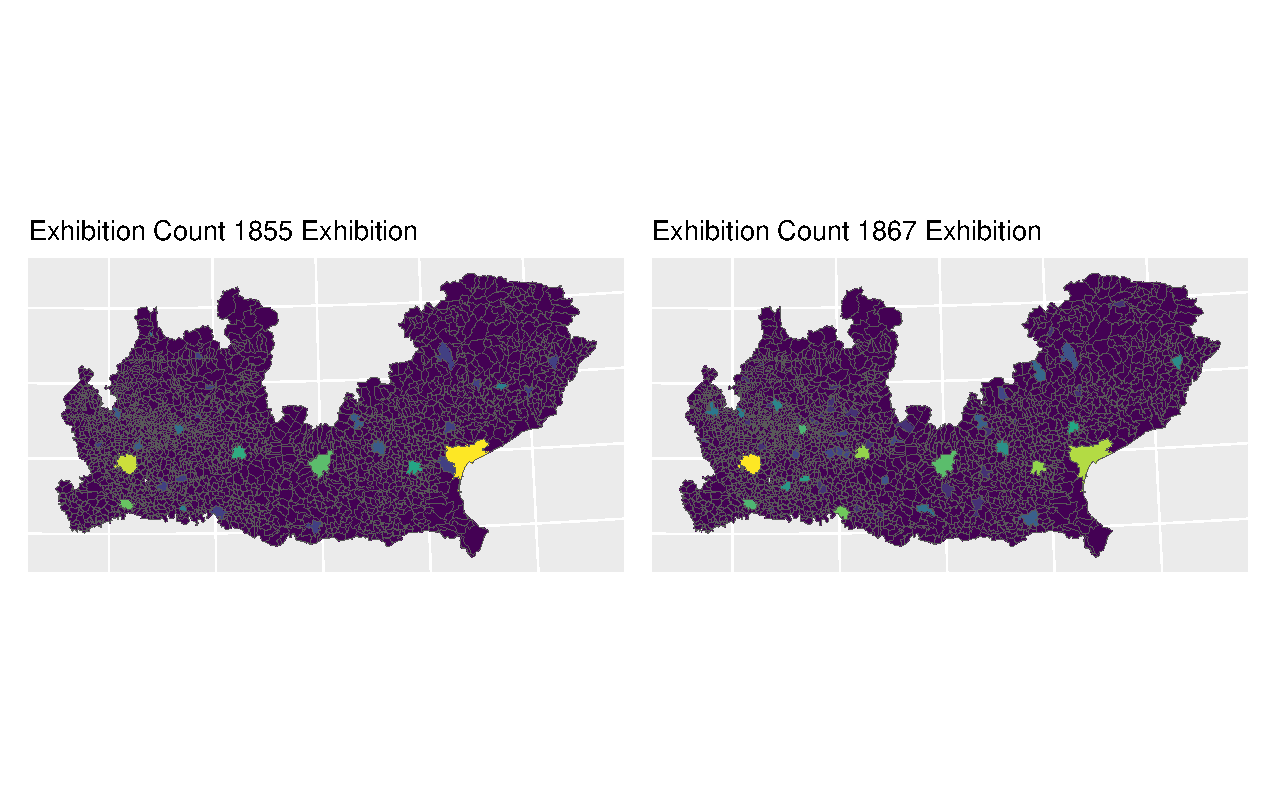
\includegraphics[width=1.0\linewidth]{graphs/exhibition_count.pdf}
    \caption{Geographical Distribution of Exhibitions in 1855 and 1867}
    \label{fig:exhibition_count}
\end{figure}


